\documentclass[11pt, a5paper, parskip=half-, DIV=12]{scrartcl}

\usepackage{../endeavour}
\usepackage{../endeavour_book}

\version{0.1}

\begin{document}
% Colour Cover
\thispagestyle{plain}
\AddToShipoutPictureBG{
\begin{tikzpicture}[remember picture, overlay]
	\node () at (current page.center) {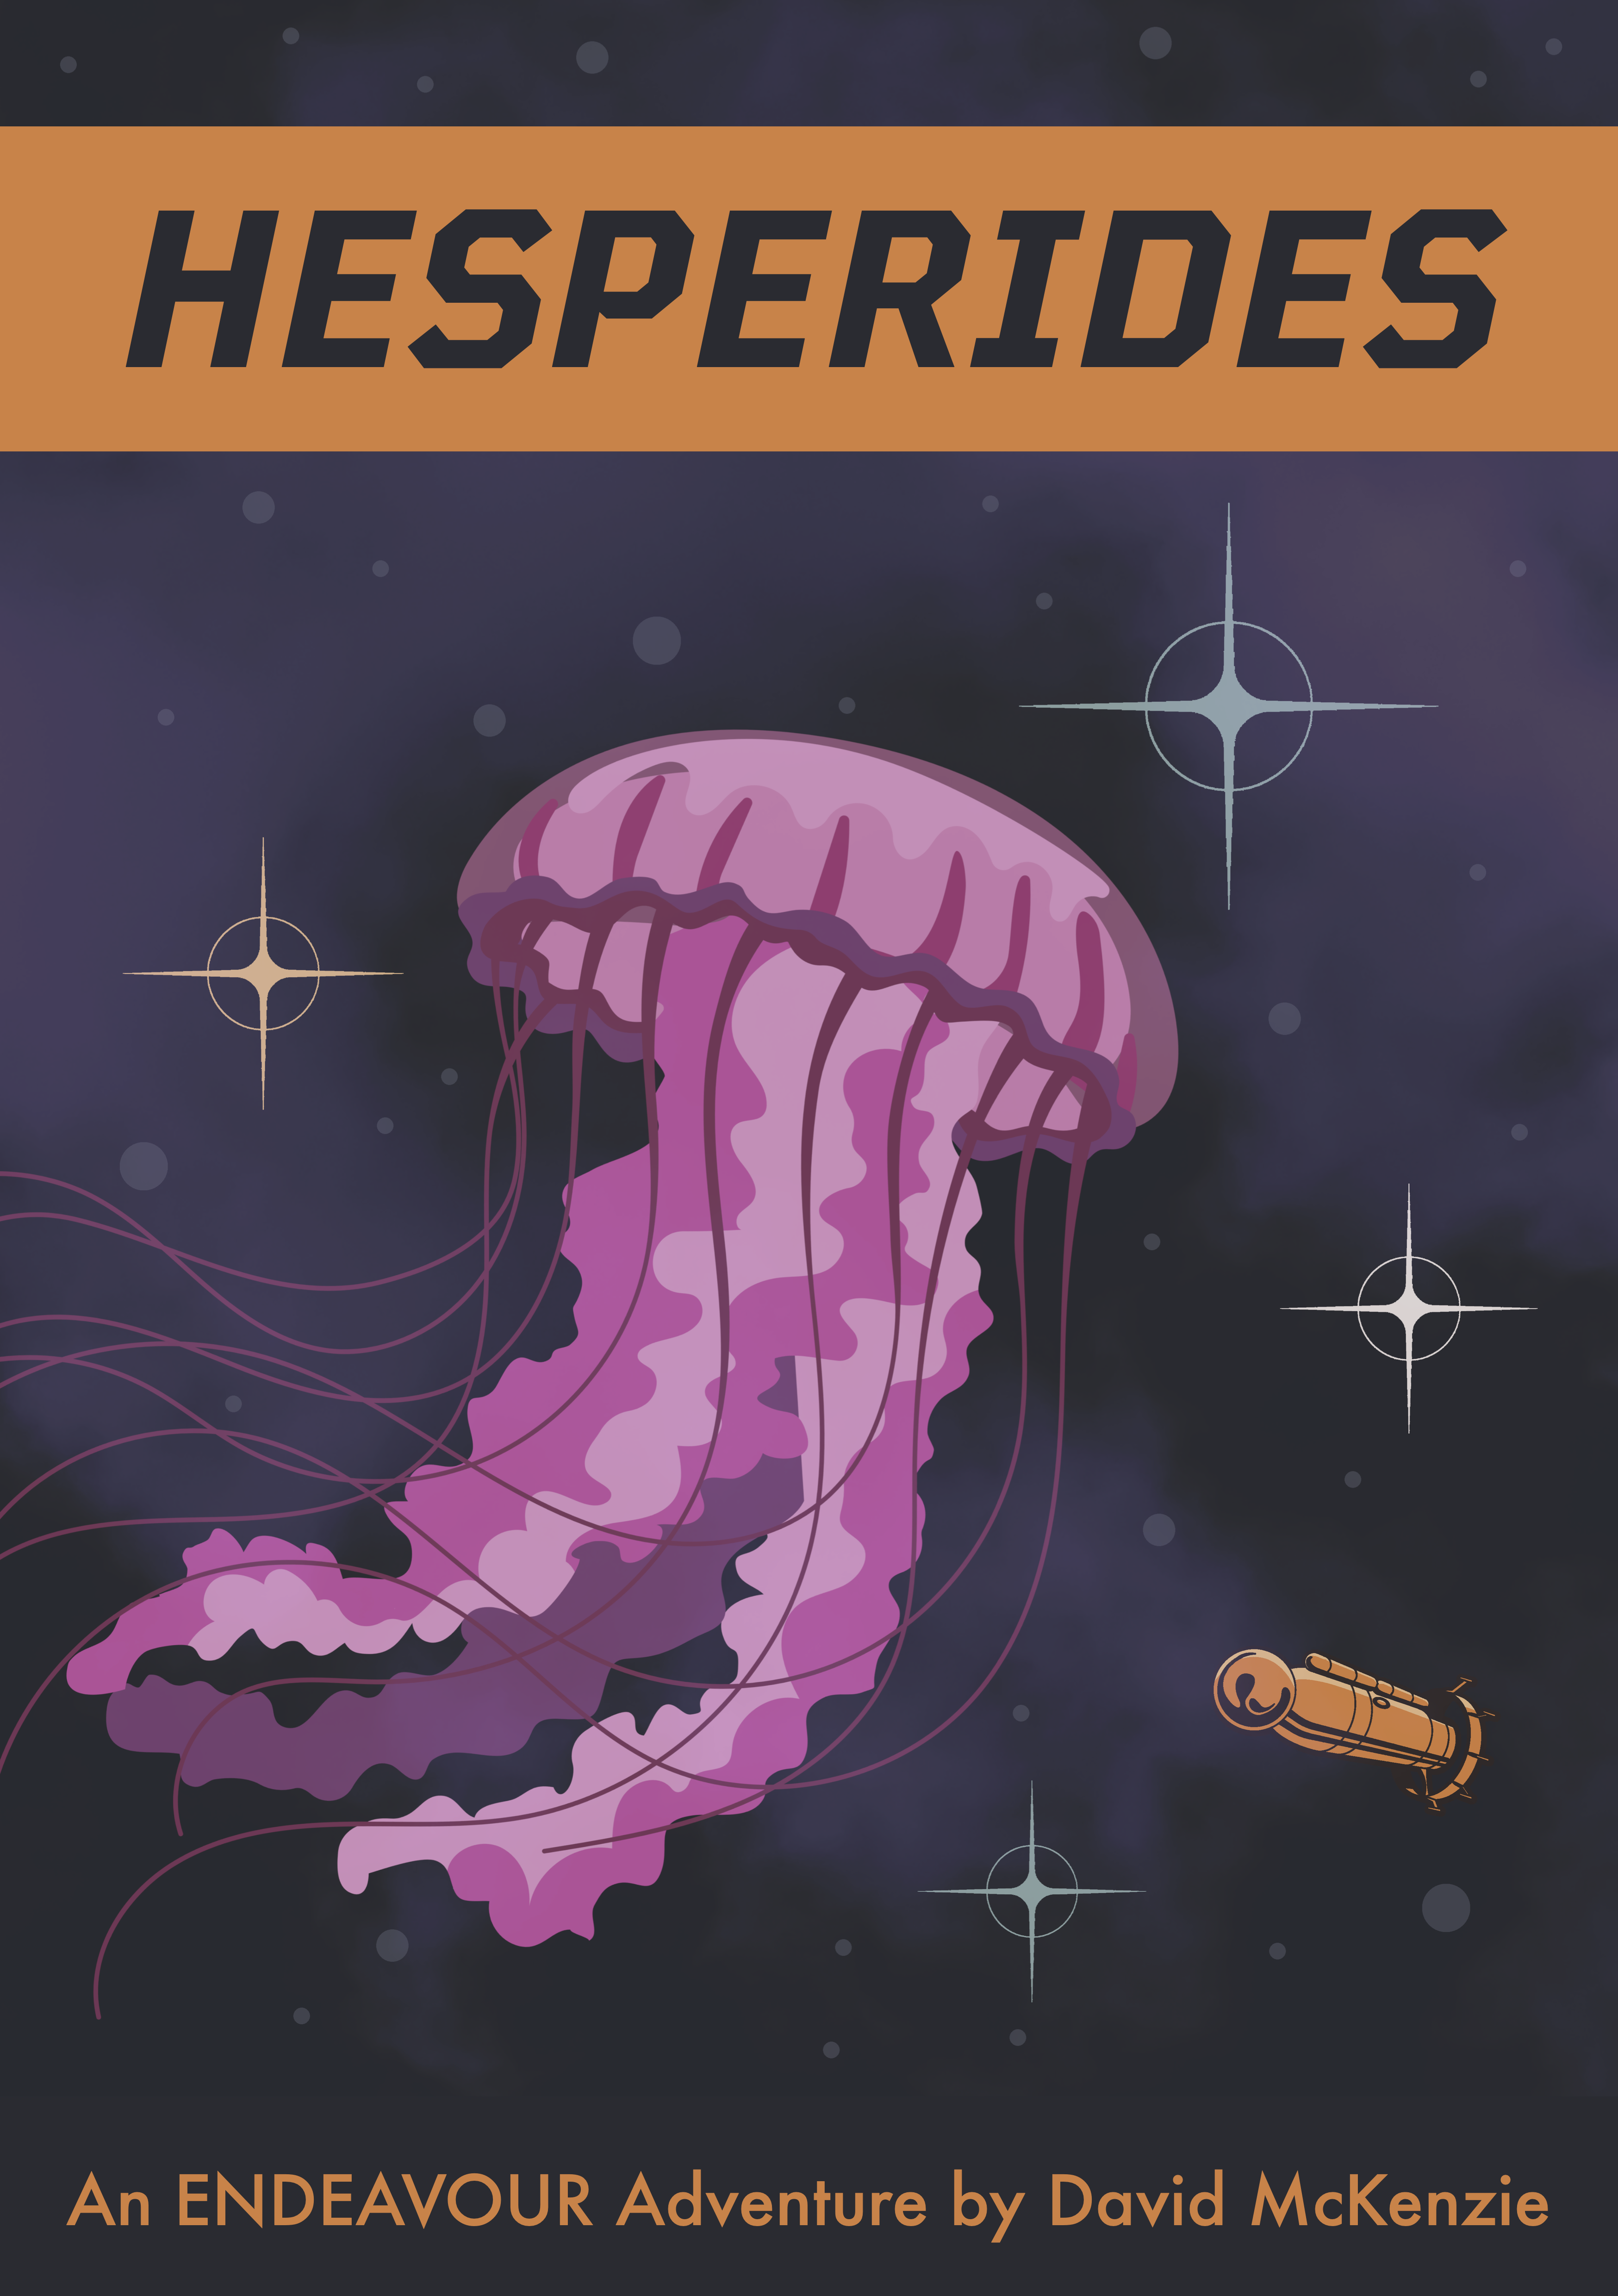
\includegraphics[width=\pagewidth, height=\pageheight]{Images/hesperides_cover.png}};
\end{tikzpicture}
}
{
\colorlet{headfootcolor}{LCARS_ORANGE}
\phantom{a}

\newpage
}

\ClearShipoutPicture
\AddToShipoutPictureBG{
	\begin{tikzpicture}[remember picture, overlay]
	\pic () at (current page.center) {starfield};
		\node[endeavour_box, minimum width=12.6cm, minimum height=18.8 cm] at (current page.center) {};
	\end{tikzpicture}
}

\setcounter{page}{1}
\setmainfont{TeX Gyre Schola}
\normalsize
\raggedright

\section*{Hesperides}
\textit{\textbf{Captain's Log:} We have been granted the rare opportunity to visit the dense nebula known as the Hesperides stellar nursery. The gardeners of this nursery \textemdash{} the Nidar of the Seventh Mother \textemdash{} have requested that we take steps to minimize our impact on the natural processes of the nebula.}

\textit{In order to facilitate this request, the Nidar have agreed to enhance our shields with some of their own technology. I will be hosting a luncheon for the Seventh Mother's command crew while their engineers oversee the shield modifications.}

\subsection*{Arrival}
Representing the Nidar aboard the Endeavour are a small diplomatic delegation led by \textbf{Sieto} and an engineering team lead by \textbf{Maraq}.
\textbf{Vassen} commands the Seventh Mother.

\subsubsection*{Bifurcation Point}
\begin{itemize}
	\item \textit{Will you take advantage of the opportunity to learn more about the Nidar by attending the captain's luncheon?} 
%	\textbf{Leadership \& Negotiation} vs. \textbf{Sieto}.
	\item \textit{Or will you work with the Maraq's engineering team to make the modifications to the Endeavour's shields?} 
%	\textbf{Operations \& Engineering} vs. \textbf{Maraq}.  
\end{itemize}

The Endeavour and the Seventh Mother are trapped in a time loop. Each iteration of the loop begins as the Nidar arrive at the Endeavour and ends several hours later when the Seventh Mother is destroyed by a ``ripple'' of exotic energy that emanates from somewhere within the nebula nearby.

%The crew of the Endeavour are aware of their predicament and their memories persist from one iteration of the loop to the next.  The Nidar experience the situation differently; their memories reset at the beginning of each iteration of the loop.

Any characters who decided to assist with the shield modifications during the first iteration of the loop will be aware of their predicament and their memories will persist from one iteration of the loop to the next. All other characters will experience the situation differently; their memories will reset at the beginning of each iteration of the loop.
\newpage

\subsection*{Trials}
During each iteration of the time loop, each character will have time to address one of the following Trials.
Each Trial grants an Advantage die for the Crisis. Each time you prevail in a Trial, increase the size of its die (1d6 $\Longrightarrow$ 1d8 $\Longrightarrow$ 1d10). 

\subsubsection*{Cultural Exchange}
The senior staff of the Seventh Mother
are aboard the Endeavour to learn more about the ICF.
%know more than anyone about the stellar nebula.
If you can gain their trust, warnings of impending danger are more likely to be well received. \textit{Can you find common ground with the Nidar?} \textbf{Leadership \& Negotiation} vs. \textbf{Sieto}.

\subsubsection*{Lower Decks}
With so many of its crew aboard the Endeavour, the Seventh Mother is unable to react quickly enough when danger arises. If you can convince Vassen to take preemptive action, the Nidar may be able to save themselves. \textit{Can you convince Vassen to act decisively?} \textbf{Strategy \& Tactics} vs. \textbf{Vassen}.

\subsubsection*{Temporal Mechanics}
Maraq is an expert in Nidar technology and complex shield harmonics but knows very little about temporal mechanics.
%Together, you may be able to find a way to break out of the time loop.
\\ \textit{Can you work together to determine the cause of the time loop?} \textbf{Science \& Medicine} vs. \textbf{The Time Loop (2d12)}. You must prevail at this Trial before you can break out of the time loop.

\subsection*{Crisis}
\begin{itemize}
	\item \textit{Will you proceed to the next iteration?} \\ \textbf{Complications:} All characters mark \tikz[baseline=-0.75ex, scale=0.85, transform shape]{\pic {stress_circle};} (Stress). 
	\item \textit{Or will you break out of the time loop?} \\ \textbf{Difficulty:} The target number for each Threat is \textbf{18}. \\ \textbf{Threats:} The Seventh Mother is destroyed, its crew lost. Future star formation within the stellar nursery is disrupted. The Endeavour becomes unstuck in time.
\end{itemize}
\newpage

\subsection*{Characters}
\begin{description}
	\item[Sieto (d10):] Captain of the Seventh Mother (d10), \\ Acts With Confidence (d8), Passionate (d8), Decisive (d8).
	\item[Vassen (d8):] First Officer of the Seventh Mother (d8), \\ Endures With Patience (d8), Tolerant (d8),  Cautious (d8).
	\item[Maraq (d8):] Chief Engineer of the Seventh Mother  (d8), Fixes What Is Broken (d8), Curious (d8), Analytical (d8).
\end{description}

\subsection*{Places}
\begin{description}
	\item[Seventh Mother:] A huge, jellyfish-like spacefaring entity that coasts through the Hesperides nebula.
	\item[Main Engineering:] A collection of computer consoles and workstations deep in the heart of the Endeavour. The Seventh Mother's tentacles snake throughout the area.
	\item[Captain's Mess:] A formal dining room used by Captain Darcy to entertain guests aboard the Endeavour.
\end{description}

\subsection*{Mysteries}
\begin{description}
%	\item[The Nidar experience time nonlinearly.] \phantom{} \\ The Nidar cannot tell that they are in a time loop. Their memories do not persist from one iteration to the next. \textit{test?}
	\item[The Seventh Mother is a living space ship.] \phantom{} \\ Countless generations of the Nidar have worked aboard the Seventh Mother. They are devoted to cultivating the new stars which are forming in the stellar nursery. \\ \textit{Are there any other Mothers elsewhere in the galaxy? \\ Did the Nidar create the Seventh Mother (or vice versa)?}
	\item[The Nidar use light and color to communicate.] \phantom{a} \\ The Nidar cannot hear. Their language is comprised of intricate three-dimensional, full-color displays that slowly evolve over time. \textit{How does the way in which the Nidar communicate affect their perception of time? How do they communicate when they cannot see one another?}
\end{description}

\newpage

\section*{Acknowlegements}
Much of the look and feel of \ENDEAVOUR{} is derived from its art, all of which was created by \textbf{svekloid}. This art was assembled from multiple collections available online at \href{http://shutterstock.com}{shutterstock.com} and then modified by Michael Purcell.  

\subsection*{Playtesters} \label{subsection:playtesters}
The following people helped to create \ENDEAVOUR{} by playing early versions of the game and providing invaluable feedback.\vspace{-1.75ex}
\begin{multicols}{2}
\begin{itemize}[noitemsep]
  \item Keydan Bruce
  \item Dannielle Harden
  \item Andrew Hellyer
%  \item Sarah Hewat
%  \item Scott Joblin
%  \item Sen-Foong Lim
  \item David McKenzie
%  \item Holly Moore
  \item Paul Murray
%  \item David Purcell
%  \item Heidi Purcell
  \item Kira Purcell
  \item Luke Purcell
  \item Meagan Purcell
%  \item Steve Purcell
%  \item Jason Stark
  \item Jo Stephenson
%  \item Pieter Vismans
  \item Brett Witty
  \item Bevis Worcester
  \item Evan Worcester
\end{itemize}
\end{multicols}

\subsection*{Design Tools} \label{subsection:design-tools}
The following tools were used to create this document:
\begin{description}[font=\normalfont\textbullet\space, noitemsep, topsep=-1ex]
	\item[LuaLaTeX:] Typesetting and layout.
	\item[TikZ:] Diagrams and art.
\end{description}
\vspace{1ex}
The fonts used are {\setmainfont{TT Mussels-BoldItalic} TT~Mussels~Bold~Italic},  \textsf{Futura}, and TeX~Gyre~Schola (cf. Century Schoolbook).

\vfill

\begin{tabular}{@{}m{7.775cm}@{\hspace*{0.375cm}}>{\centering\arraybackslash}m{2.6cm}@{}}
\textbf{Contact:} \href{mailto:endeavour.ttrpg@gmail.com}{endeavour.ttrpg@gmail.com}\newline \phantom{This is a test, only a test.} \newline \footnotesize{For use with the \textsc{Paragon} system, ©2020\newline \textbf{John Harper \& Sean Nittner}. \href{http://agon-rpg.com}{AGON-RPG.com}} & \includegraphics[scale=0.175]{Images/paragon_logo_mark.png} \\[5ex]
\footnotesize{This work is licensed under a Creative Commons \newline ``Attribution-ShareAlike 4.0 International'' license.} & \Huge{\doclicenseIcon}
\end{tabular}

\newpage

\thispagestyle{empty}

\tikzset{starfield/.pic={
	\node () at (current page.center) {
\includegraphics[width=\pagewidth, height=\pageheight]{Images/starfield.png}};
}}

\ClearShipoutPicture
\AddToShipoutPictureBG{
	\begin{tikzpicture}[remember picture, overlay]
	\pic () at (current page.center) {starfield};
	\end{tikzpicture}
}

\phantom{a}

\end{document}